\documentclass[xelatex,aspectratio=169]{beamer}

\hfuzz=10pt
\vfuzz=10pt

% Theme
\usetheme{htw}
\setbeamertemplate{navigation symbols}{}
\setbeamertemplate{theorems}[numbered]
\setbeamercovered{transparent}

%\logo{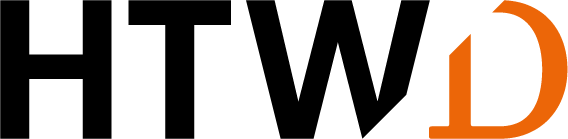
\includegraphics[height=0.5cm]{HTWD_color.png}}

% Packages
\usepackage{polyglossia}
\setmainlanguage{german}
\setotherlanguage{english}

\usepackage[bigfiles]{pdfbase}
\ExplSyntaxOn
\NewDocumentCommand\embedvideo{smm}{
\group_begin:
\leavevmode
\tl_if_exist:cTF{file_\file_mdfive_hash:n{#3}}{
  \tl_set_eq:Nc\video{file_\file_mdfive_hash:n{#3}}
}{
  \IfFileExists{#3}{}{\GenericError{}{File~`#3'~not~found}{}{}}
  \pbs_pdfobj:nnn{}{fstream}{{}{#3}}
  \pbs_pdfobj:nnn{}{dict}{
    /Type/Filespec/F~(#3)/UF~(#3)
    /EF~<</F~\pbs_pdflastobj:>>
  }
  \tl_set:Nx\video{\pbs_pdflastobj:}
  \tl_gset_eq:cN{file_\file_mdfive_hash:n{#3}}\video
}
%
\pbs_pdfobj:nnn{}{dict}{
  /Type/RichMediaInstance/Subtype/Video
  /Asset~\video
  /Params~<</FlashVars (
  source=#3&
  skin=SkinOverAllNoFullNoCaption.swf&
  skinAutoHide=true&
  skinBackgroundColor=0x5F5F5F&
  skinBackgroundAlpha=0.75
  )>>
}
%
\pbs_pdfobj:nnn{}{dict}{
/Type/RichMediaConfiguration/Subtype/Video
/Instances~[\pbs_pdflastobj:]
}
%
\pbs_pdfobj:nnn{}{dict}{
/Type/RichMediaContent
/Assets~<<
/Names~[(#3)~\video]
>>
/Configurations~[\pbs_pdflastobj:]
}
\tl_set:Nx\rmcontent{\pbs_pdflastobj:}
%
\pbs_pdfobj:nnn{}{dict}{
  /Activation~<<
  /Condition/\IfBooleanTF{#1}{PV}{XA}
  /Presentation~<</Style/Embedded>>
  >>
  /Deactivation~<</Condition/PI>>
}
%
\hbox_set:Nn\l_tmpa_box{#2}
\tl_set:Nx\l_box_wd_tl{\dim_use:N\box_wd:N\l_tmpa_box}
\tl_set:Nx\l_box_ht_tl{\dim_use:N\box_ht:N\l_tmpa_box}
\tl_set:Nx\l_box_dp_tl{\dim_use:N\box_dp:N\l_tmpa_box}
\pbs_pdfxform:nnnnn{1}{1}{}{}{\l_tmpa_box}
%
\pbs_pdfannot:nnnn{\l_box_wd_tl}{\l_box_ht_tl}{\l_box_dp_tl}{
  /Subtype/RichMedia
  /BS~<</W~0/S/S>>
  /Contents~(embedded~video~file:#3)
  /NM~(rma:#3)
  /AP~<</N~\pbs_pdflastxform:>>
  /RichMediaSettings~\pbs_pdflastobj:
  /RichMediaContent~\rmcontent
}
\phantom{#2}
\group_end:
}
\ExplSyntaxOff


\usepackage{graphicx}
\usepackage[export]{adjustbox}
\usepackage{animate}
%\usepackage[dvipdfmx]{movie15_dvipdfmx}
\usepackage{media9}
\usepackage{tabularx}
\usepackage{colortbl}
\usepackage{booktabs}
\usepackage{makecell}
\usepackage{ltablex}
\usepackage{array}
\usepackage{multirow}
\usepackage{amsmath}
\usepackage{amsthm}
%\renewcommand{\arraystretch}{1.5}
\newcolumntype{L}[1]{>{\raggedright\let\newline\\\arraybackslash\hspace{0pt}}p{#1}}
\newcolumntype{C}[1]{>{\centering\let\newline\\\arraybackslash\hspace{0pt}}p{#1}}
\newcolumntype{R}[1]{>{\raggedleft\let\newline\\\arraybackslash\hspace{0pt}}p{#1}}
%\renewcommand\thesatz{\arabic{section}.\arabic{theorem}}
\makeatletter
\@addtoreset{theorem}{lecture}
\makeatother

\newtheorem{satz}{Satz}[section]
\newtheorem{lem}{Lemma}[section]
\newtheorem{beh}{Behauptung}[section]
\newtheorem{define}{Definition}[section]
\numberwithin{equation}{section}
\usepackage{ragged2e}
\usepackage{etoolbox}

\usepackage{color}
\usepackage{colortbl}
\definecolor{hellgrau}{rgb}{0.85,0.85,0.85}
\definecolor{hellrot}{rgb}{1,0.7,0.7}

\usepackage{tikz}
\usetikzlibrary{shapes,arrows.meta,calc,arrows,positioning,patterns,tikzmark}
%\usepackage{tikz-uml}
\usepackage{pgfplots}  % for elliptic curves (part 8)
\pgfplotsset{compat=1.18}
\usepackage{pgffor}
\usepackage{pgfmath-xfp}
\tikzset{>=latex}
\tikzset{
  invisible/.style={opacity=0},
  visible on/.style={alt={#1{}{invisible}}},
  alt/.code args={<#1>#2#3}{%
      \alt<#1>{\pgfkeysalso{#2}}{\pgfkeysalso{#3}} % \pgfkeysalso doesn't change the path
    },
}

\usepackage{paralist}

\usepackage{url}
\def\UrlBreaks{\do\/\do-}
\PassOptionsToPackage{hyphens}{url}\usepackage{hyperref}

\usepackage[normalem]{ulem} % gestrichelte Unterstreichung (\dashuline{})
\usepackage{cancel}

\makeatletter
\renewcommand{\itemize}[1][]{%
  \beamer@ifempty{#1}{}{\def\beamer@defaultospec{#1}}%
  \ifnum \@itemdepth >2\relax\@toodeep\else
    \advance\@itemdepth\@ne
    \beamer@computepref\@itemdepth% sets \beameritemnestingprefix
    \usebeamerfont{itemize/enumerate \beameritemnestingprefix body}%
    \usebeamercolor[fg]{itemize/enumerate \beameritemnestingprefix body}%
    \usebeamertemplate{itemize/enumerate \beameritemnestingprefix body begin}%
    \list
    {\usebeamertemplate{itemize \beameritemnestingprefix item}}
    {\def\makelabel##1{%
        {%
            \hss\llap{{%
                  \usebeamerfont*{itemize \beameritemnestingprefix item}%
                  \usebeamercolor[fg]{itemize \beameritemnestingprefix item}##1}}%
          }%
      }%
    }
  \fi%
  \beamer@cramped%
  \justifying% NEW
  %\raggedright% ORIGINAL
  \beamer@firstlineitemizeunskip%
}
\makeatother

\apptocmd{\frame}{}{\justifying}{}

\renewcommand\theadfont{\bfseries\sffamily}
\usepackage{ragged2e}
\usepackage{newpxtext}

\setsansfont{texgyreheros}[
  Scale=MatchLowercase,
  UprightFont=*-regular,
  BoldFont=*-bold,
  ItalicFont=*-italic,
  BoldItalicFont=*-bolditalic,
]

% Title
\usepackage[usetransparent=false]{svg}
% Import references
\usepackage[backend=biber,style=numeric,sorting=none]{biblatex}
\addbibresource{references.bib}

%\AtBeginSection[]{
%  \begin{frame}
%    \vfill
%    \centering
%    \begin{beamercolorbox}[sep=8pt,center,shadow=true,rounded=true]{title}
%      \usebeamerfont{title}\thesection.~\secname\par%
%    \end{beamercolorbox}
%    \vfill
%  \end{frame}
%}

\makeatletter
\newenvironment{noheadline}{
  \setbeamertemplate{headline}{}
  \addtobeamertemplate{frametitle}{\vspace*{-0.9\baselineskip}}{}
}{}
\makeatother


\usepackage{xcolor}
\usepackage{algorithm}
\usepackage[linesnumbered,ruled,lined,commentsnumbered,algo2e,ngerman,ngermankw]{algorithm2e}
\usepackage{algorithmic}
\usepackage{caption}
\usepackage[newfloat]{minted}
\captionsetup[listing]{position=top}
\definecolor{mintedbg}{HTML}{282828}
\setminted{
  breaklines=true,
  bgcolor=mintedbg,
  style=monokai,
  formatcom=\color{white}
}
\usepackage{etoolbox}
\makeatletter
% replace \medskip before and after the box with nothing, i.e., remove it
\patchcmd{\minted@colorbg}{\medskip}{}{}{}
\patchcmd{\endminted@colorbg}{\medskip}{}{}{}
\makeatother

\renewcommand{\theFancyVerbLine}{\textcolor{black}{\arabic{FancyVerbLine}}}

\usepackage{pifont}
\newcommand{\cmark}{\ding{51}}%
\newcommand{\xmark}{\ding{55}}%

\newenvironment{changemargin}[2]{%
  \begin{list}{}{%
      \setlength{\topsep}{0pt}%
      \setlength{\leftmargin}{#1}%
      \setlength{\rightmargin}{#2}%
      \setlength{\listparindent}{\parindent}%
      \setlength{\itemindent}{\parindent}%
      \setlength{\parsep}{\parskip}%
    }%
    \item[]}{\end{list}}


\usepackage{csquotes}

% Title
\title{Fortgeschrittenes Python}
\author{Prof. Dr. Lukas Iffländer}
\institute{HTW Dresden}
\date{}
\usepackage{svg}

% Begin document
\begin{document}

% Title slide
\begin{frame}
    \titlepage
\end{frame}

\begin{frame}{Datentypen von Anordnungen}
    Python bietet eine Vielzahl von Datentypen, um Anordnungen von Daten zu speichern. Die wichtigsten sind:
    \begin{description}
        \item[Listen] lineare Anordnungen von Elementen, die veränderbar sind
        \item[Tupel] lineare Anordnungen von Elementen, die unveränderbar sind
        \item[Sets] ungeordnete Sammlungen von einzigartigen Elementen
        \item[Dictionaries] ungeordnete Sammlungen von Schlüssel-Wert-Paaren
    \end{description}
\end{frame}

\section{Listen}

\begin{frame}{Listen}
    \begin{block}{Definition}
        Listen sind geordnete Sammlungen von Elementen, die veränderbar sind. Sie können verschiedene Datentypen enthalten und bieten eine Vielzahl von Methoden zur Manipulation der Daten.lineare Anordnung von Elementen, die oftmals gleichen Typ besitzen, aber auch unterschiedliche Typen aufweisen dürfen.
        Auf Listen kann indiziert zugegriffen werden.
    \end{block}
\end{frame}

\begin{frame}{Listen}{Beispiel}
    \inputminted{python}{src/listen_overview.py}
\end{frame}

\begin{frame}{Listen}{Funktionen}
    Für Listen gibt es in python eingebaute Funktionen, die eine Vielzahl von Operationen ermöglichen. Hier sind einige der wichtigsten:
    \inputminted{python}{src/listen_funktionen.py}
\end{frame}

\begin{frame}{Listen}{Methoden}
    \begin{tabularx}{\textwidth}{lX}
        \toprule
        \textbf{Methode} & \textbf{Beschreibung}                                              \\
        \midrule
        append()         & Fügt ein Element am Ende der Liste hinzu.                          \\
        extend()         & Fügt mehrere Elemente am Ende der Liste hinzu.                     \\
        insert()         & Fügt ein Element an einer bestimmten Position in der Liste ein.    \\
        remove()         & Entfernt das erste Vorkommen eines Elements aus der Liste.         \\
        pop()            & Entfernt und gibt das Element an einer bestimmten Position zurück. \\
        clear()          & Entfernt alle Elemente aus der Liste.                              \\
        index()          & Gibt den Index des ersten Vorkommens eines Elements zurück.        \\
        count()          & Gibt die Anzahl der Vorkommen eines Elements in der Liste zurück.  \\
        sort()           & Sortiert die Elemente in aufsteigender Reihenfolge.                \\
        reverse()        & Kehrt die Reihenfolge der Elemente in der Liste um.                \\
        copy()           & Gibt eine flache Kopie der Liste zurück.                           \\
        \bottomrule
    \end{tabularx}

\end{frame}

\begin{frame}{Listen}{Mehrdimensionale Listen}
    Matrizen und höherdimensionale Anordnungen können durch verschachtelte Listen erzeugt werden.
    \inputminted[lastline=2]{python}{src/listen_mehrdimensional.py}

    Zeilenauswahl durch Zugriff auf entsprechende Unterliste
    \inputminted[firstline=4,lastline=4]{python}{src/listen_mehrdimensional.py}

    Elementauswahl durch Indizierung mit Zeilenindex, Spaltenindex
    \inputminted[firstline=6,lastline=6]{python}{src/listen_mehrdimensional.py}

    Eine Spaltenauswahl ist  etwas umständlichler, hier Spalte mit index 2:
    \inputminted[firstline=8,lastline=8]{python}{src/listen_mehrdimensional.py}
\end{frame}

\begin{frame}{Listen}{List Comprehensions}
    List Comprehensions sind eine elegante Möglichkeit, Listen zu erstellen und zu manipulieren. Sie ermöglichen es, eine neue Liste aus einer bestehenden Liste zu generieren, indem man eine Ausdrucksform verwendet, die die Elemente der bestehenden Liste durchläuft und sie in eine neue Liste umwandelt.

    \begin{itemize}
        \item \texttt{list()} erzeugt eine Liste aus einem Ausdruck
    \end{itemize}


    \inputminted[lastline=8]{python}{src/listen_comprehensions.py}
\end{frame}

\section{Tupel}

\begin{frame}{Tupel}
    \begin{block}{Definition}
        Tupel sind unveränderbare Anordnungen von Elementen mit Reihung.
    \end{block}

    \inputminted[lastline=4]{python}{src/tupel_overview.py}

    Zugriff auf Element mit numerischem Index (wie bei Listen)

    \inputminted[firstline=6]{python}{src/tupel_overview.py}

    \begin{block}{Eigenschaften}
        \begin{itemize}
            \item feste Länge
            \item Elemente sind unveränderbar
            \item Tupel muss bei Änderungen neu zugewiesen werden
        \end{itemize}

    \end{block}

\end{frame}

\begin{frame}{Tupel}{Verschachtelung}
    \begin{block}{Verschachtelte Tupel}
        \small
        \inputminted[lastline=5]{python}{src/tupel_nested.py}
    \end{block}
    \vspace{-5pt}
    \begin{alertblock}{Tupel sind nicht änderbar}
        \small
        Eine nachträgliche Änderung der Werte in einem Tupel ist nicht möglich.
        \vspace{-5pt}
        \inputminted[firstline=7]{python}{src/tupel_nested.py}

    \end{alertblock}

\end{frame}

\begin{frame}{Tupel}{Tupel und Listen}
    \begin{block}{Tupel of Lists}
        Tupel können Listen enthalten (die dann veränderbar sind):
        \inputminted[lastline=1]{python}{src/tupel_und_listen.py}
    \end{block}
    \begin{block}{List of Tuples}
        Listen können Tupel enthalten:
        \inputminted[firstline=4,lastline=4]{python}{src/tupel_und_listen.py}
    \end{block}
    \begin{block}{Zip-Funktion}
        Die \texttt{zip()}-Funktion kann zwei Listen zu einer Liste von Tupeln kombinieren:
        \inputminted[firstline=7,lastline=7]{python}{src/tupel_und_listen.py}
    \end{block}
\end{frame}

\begin{frame}{Sets}
    \begin{block}{Definition}
        Sets bilden ungeordnete Mengen ab.
        \begin{itemize}
            \item Jedes Element kann nur einmmal im Set vorkommen.
            \item Die Reihenfolge der Elemente ist nicht festgelegt, ein Zugriff über den Index ist nicht möglich.
        \end{itemize}

    \end{block}
    \begin{exampleblock}{Beispiel}
        \inputminted{python}{src/sets_overview.py}
    \end{exampleblock}

    Basisoperationen sind:
    \begin{itemize}
        \item \texttt{add()} - fügt ein Element hinzu
        \item \texttt{remove()} - entfernt ein Element
    \end{itemize}

\end{frame}

\begin{frame}{Sets}{Beispiel}
    \inputminted{python}{src/sets_example.py}
\end{frame}

\begin{frame}{Sets}{Mengenoperationen}
    Mengen können mit mengenalgebraischen Operationen verknüpft werden:
    \begin{itemize}
        \item [\texttt{|}] Vereinigung
        \item [\texttt{\&}] Schnittmenge
        \item [\texttt{-}] Differenz
        \item [\texttt{\^}] Unterschiedliche Elemente, die nur in einer Mengen vorkommen
    \end{itemize}

    \inputminted[lastline=7]{python}{src/sets_operations.py}

\end{frame}

\section{Dictionaries}

\begin{frame}{Dictionaries}
    \begin{block}{Definition}
        Dictionaries sind ungeordnete Sammlungen von Schlüssel-Wert-Paaren. Sie sind veränderbar und ermöglichen den schnellen Zugriff auf Werte über ihre Schlüssel.
    \end{block}

    \begin{block}{Definition}
        Schlüssel sind eindeutige Merkmale, über die Elemente gefunden werden können. Beispiele sind Matrikelnummern oder ISBN-Nummern von Büchern.
    \end{block}

    \begin{exampleblock}{Beispiel}
        \inputminted[lastline=6]{python}{src/dictionaries_overview.py}
    \end{exampleblock}
\end{frame}

\begin{frame}{Dictionaries}{Zugriff}
    Das Prüfen, ob ein Element enthalten ist, wird über den Schlüssel durchgeführt:

    \mintinline{python}|key in dictionary| $\rightarrow$ \mintinline{python}|True| oder \mintinline{python}|False|.\\

    \begin{exampleblock}{Beispiel}
        \inputminted[firstline=8,lastline=9]{python}{src/dictionaries_overview.py}
    \end{exampleblock}

    Durchlaufen aller Elementer erfolgt mit dem Befehl \mintinline{python}|for key in dictionary|.

    \begin{exampleblock}{Beispiel}
        \inputminted[firstline=11,lastline=12]{python}{src/dictionaries_overview.py}
    \end{exampleblock}

\end{frame}

\begin{frame}{Dictionaries}{Operationen I}
    Löschen eines Elements erfolgt über den Befehl \mintinline{python}|del dictionary[key]|.
    \begin{exampleblock}{Beispiel}
        \inputminted[firstline=14,lastline=14]{python}{src/dictionaries_overview.py}
    \end{exampleblock}

    Einfügen eines neuen Elements und ändern eines bestehenden Elements erfolgt über den Befehl \mintinline{python}|dictionary[key] = value|.

    \begin{exampleblock}{Beispiel}
        \inputminted[firstline=16,lastline=17]{python}{src/dictionaries_overview.py}
    \end{exampleblock}

\end{frame}
\begin{frame}{Dictionaries}{Operationen II}
    \begin{itemize}
        \item \mintinline{python}|len(dictionary)| gibt die Anzahl der Elemente zurück.
        \item \mintinline{python}|dictionary.clear()| entfernt alle Elemente.
        \item \mintinline{python}|variable = dictionary.get(key)| gibt den Wert des Schlüssels zurück. Im Gegensatz zu \mintinline{python}|dictionary[key]| wird kein Fehler geworfen, wenn der Schlüssel nicht existiert, sondern \mintinline{python}|None| zurückgegeben.
        \item \mintinline{python}|dictionary.keys()| gibt eine Liste der Schlüssel im Dictionary zurück.
        \item \mintinline{python}|dictionary.values()| gibt eine Liste der Werte im Dictionary zurück.
        \item \mintinline{python}|dictionary.items()| gibt eine Liste der Schlüssel-Wert-Paare im Dictionary zurück.
    \end{itemize}

\end{frame}

\begin{frame}{Dictionaries}{Beispiel I}
    \begin{exampleblock}{Beispiel}
        \inputminted[firstline=1,lastline=11]{python}{src/dictionaries_example.py}
    \end{exampleblock}
\end{frame}
\begin{frame}{Dictionaries}{Beispiel II}
    \begin{exampleblock}{Beispiel}
        \inputminted[firstline=13,lastline=18]{python}{src/dictionaries_example.py}
    \end{exampleblock}
\end{frame}
\begin{frame}{Dictionaries}{Beispiel III}
    \vspace{-.2cm}
    \begin{exampleblock}{Beispiel}
        \inputminted[firstline=21,lastline=33]{python}{src/dictionaries_example.py}
    \end{exampleblock}
\end{frame}
\begin{frame}{Dictionaries}{Beispiel IV}
    \begin{exampleblock}{Beispiel}
        \inputminted[firstline=36,lastline=39]{python}{src/dictionaries_example.py}
    \end{exampleblock}
\end{frame}

\section{Entscheidungshilfe}

\begin{frame}{Wann welche Datenstruktur?}

    \begin{block}{Tupel}
        Inhaltlich verbundene Datenelement (z. B. Datensatz), Anordnung ändert sich nicht während der Verarbeitung
    \end{block}

    \begin{block}{Set}
        Anordnung von Elementen ohne Doppelungen, ohne Bezug auf die Reihenfolge
    \end{block}

    \begin{block}{Liste}
        Wertereihen, die in einer bestimmten Reihenfolge angeordnet sind und verändert werden können
    \end{block}

    \begin{block}{Dictionary}
        Strukturierte Wertereihen, bei denen die Werte eindeutig mit Schlüsseln verknüpft sind
    \end{block}

\end{frame}

\section{Funktionen}

\begin{frame}{Funktionen}{Rückgabetyp \texttt{none}}
    \begin{itemize}
        \item Rückgabetyp \texttt{none} bedeutet, dass die Funktion keinen Wert zurückgibt.
        \item Dies kann sowohl explizit als auch implizit geschehen.
        \item Beispiel:
              \inputminted{python}{src/functions_return_none.py}
    \end{itemize}
\end{frame}

\begin{frame}{Funktionen}{Mehrfachzuweisung}
    \begin{block}{Mehrfachzuweisung}
        \begin{itemize}
            \item In einer Zeile können mehrere Variablen gleichzeitig zugewiesen werden.
            \item Ein besonders nützlicher Sonderfall ist die Vertauschung von Variablen.
        \end{itemize}
    \end{block}
    \begin{exampleblock}
        {Beispiel}
        \inputminted[firstline=6]{python}{src/functions_multi_asign.py}
    \end{exampleblock}
\end{frame}

\begin{frame}{Funktionen}{Rückgabe mehrerer Werte}
    \vspace{-.3cm}
    \begin{block}{Rückgabe mehrerer Werte}
        \begin{itemize}
            \item Eine Funktion kann mehrere Werte zurückgeben.
            \item Diese werden in einer Liste oder einem Tupel zusammengefasst.
        \end{itemize}
    \end{block}
    \begin{exampleblock}
        {Beispiel}
        \inputminted[firstline=4, lastline=12]{python}{src/functions_multi_return.py}
    \end{exampleblock}

\end{frame}

\begin{frame}{Funktionen}{Funktionen als Argumente}
    \begin{block}{Funktionen als Argumente}
        \begin{itemize}
            \item Funktionen können als Argumente an andere Funktionen übergeben werden.
            \item Dies ermöglicht eine hohe Flexibilität und Wiederverwendbarkeit von Code.
        \end{itemize}
    \end{block}
    \begin{exampleblock}{Beispiel}
        \begin{columns}[onlytextwidth]
            \begin{column}{0.55\textwidth}
                \inputminted[firstline=1,lastline=7]{python}{src/functions_as_argument.py}
            \end{column}
            \begin{column}{0.42\textwidth}
                \begin{center}
                    Aufruf
                \end{center}
                \inputminted[firstline=10]{python}{src/functions_as_argument.py}
            \end{column}
        \end{columns}
    \end{exampleblock}

\end{frame}

\begin{frame}{Funktionen}{Funktionen als Argument}
    \begin{exampleblock}{Beispiel}
        \begin{columns}[onlytextwidth,T]
            \begin{column}{0.4\textwidth}
                \inputminted[firstline=1,lastline=10]{python}{src/functions_as_arguments_listmap.py}
            \end{column}
            \begin{column}{0.55\textwidth}
                \inputminted[firstline=13,lastline=22]{python}{src/functions_as_arguments_listmap.py}
            \end{column}
        \end{columns}
    \end{exampleblock}
\end{frame}

\begin{frame}[fragile]{Funktionen}{Funktionen als Argument}
    \begin{exampleblock}{Beispiel}
        \vspace{-.5\baselineskip}
        \begin{columns}[onlytextwidth]
            \begin{column}{0.42\textwidth}
                \begin{itemize}
                    \item Nullstellensuche für wählbare Funktionen
                          \begin{itemize}
                              \item Funktion, deren Nullstelle gesucht werden soll ist Argument
                              \item Intervallgrenzen sind ebenfalls Argumente
                          \end{itemize}
                \end{itemize}
                \smaller
                \inputminted[firstline=4, lastline=8]{python}{src/functions_nullstellen.py}
            \end{column}
            \begin{column}{0.55\textwidth}
                \smaller
                \inputminted[firstline=11,lastline=25]{python}{src/functions_nullstellen.py}
            \end{column}
        \end{columns}
    \end{exampleblock}
\end{frame}

\begin{frame}{Funktionen}{Lambda-Funktionen}
    \begin{block}{Idee}
        Wenn eine Funktion nur einmal benötigt wird, kann man diese auch als unbenannten (auch anonymen) Funktionsausdruck angeben. Das wird als lambda-Funktion bezeichnet.
    \end{block}
    \begin{exampleblock}{Beispiel}
        \inputminted[firstline=28,lastline=28]{python}{src/functions_nullstellen.py}
        Äquivalente Definition:
        \inputminted[firstline=31]{python}{src/functions_nullstellen.py}
    \end{exampleblock}

\end{frame}

\begin{frame}{Funktionen}{Lambda-Funktionen}
    \begin{block}{Syntax}
        \texttt{lambda <argumente>: <Funktionsausdruck>}
    \end{block}
    \begin{exampleblock}{Beispiel}
        \mintinline{python}|myfun = lambda x, y: x/2 * y ** 2|

        \texttt{myfun} kann als Funktionsargument übergeben werden oder direkt als \mintinline{python}|myfun(m,V)| aufgerufen werden.
    \end{exampleblock}
\end{frame}

\begin{frame}{Funktionen}{Lambda-Funktionen--beispiel}
    \begin{exampleblock}{Beispiel}
        \inputminted{python}{src/functions_lambda_example.py}
    \end{exampleblock}
\end{frame}

\begin{frame}[t]{Veränderbare und unveränderbare Objekte}{Funktionsargumente}
    \begin{alertblock}{Frage:}
        Was passiert, wenn ich eine übergebene Variable verändere?
    \end{alertblock}

    \begin{exampleblock}{Beispiel}
        \inputminted{python}{src/functions_mutable_example.py}
        \only<2->{\textbf{Antwort:} Die Variable wird verändert.}
    \end{exampleblock}

\end{frame}


\begin{frame}[t]{Veränderbare und unveränderbare Objekte}{Kopierte Objekte}
    \begin{alertblock}{Frage:}
        Was passiert, wenn ich eine übergebene Variable verändere?
    \end{alertblock}

    \begin{exampleblock}{Beispiel}
        \inputminted{python}{src/functions_copy_example.py}
        \only<2->{\textbf{Antwort:} Die Variable wird verändert.}
    \end{exampleblock}

\end{frame}

\begin{frame}{Veränderbare und unveränderbare Objekte}{Immutable}
    \begin{itemize}
        \item alle Basistypen (int, float, bool, str) und Tupel
        \item Übergaben als Argument an Funktionen sind immer Kopien. Funktionen überschreiben die Variablen nicht.
        \item Bei der Zuweisung wird eine neue Variable erstellt und der Wert kopiert.
    \end{itemize}

\end{frame}

\begin{frame}{Veränderbare und unveränderbare Objekte}{Mutable}
    \begin{itemize}
        \item Anordnungstypen (Listen, Dictionaries, Sets) und benutzerdefinierte Objekte
        \item Übergaben als Argument erfolgen als Referenz zum Original. Funktionen überschreiben die Variablen.
        \item Bei Zuweisung wird die Referenz kopiert. Die Variable zeigt auf das selbe Objekt.
    \end{itemize}
\end{frame}

\section{Listen und Funktionen}

\begin{frame}{Listen und Funktionen}
    \begin{block}{Konzept}
        Für Listen können Funktionen bzw. Lambdas übergeben werden,
        \begin{itemize}
            \item um Funktionsausführungen auf die Listenelemente elementweise zu mappen (\texttt{map()}),
            \item um Filterfunktionen zu definieren und elementweise auszuführen (\texttt{filter()}),
            \item um Reduktionsoperationen zu definieren und auszführen (\texttt{reduce()}).
        \end{itemize}
    \end{block}
\end{frame}

\begin{frame}{Listen und Funktionen}{Typen}
    \begin{description}
        \item[list()]
              \begin{itemize}
                  \item Erzeugt eine Liste aus den Argumenten
                  \item Beispiel: \mintinline{python}|list(1, 2, 3)|
              \end{itemize}
        \item[map()]
              \begin{itemize}
                  \item Wendet eine Funktion auf alle Elemente einer Liste an
                  \item Beispiel: \mintinline{python}|map(lambda x: x + 1, list(1, 2, 3))|
              \end{itemize}
        \item[filter()]
              \begin{itemize}
                  \item Filtert eine Liste basierend auf einer Bedingung
                  \item Beispiel: \mintinline{python}|filter(lambda x: x > 1, list(1, 2, 3))|
              \end{itemize}
        \item[reduce()]
              \begin{itemize}
                  \item Reduziert eine Liste auf einen einzelnen Wert
                  \item Beispiel: \mintinline{python}|reduce(lambda x, y: x + y, list(1, 2, 3))|
              \end{itemize}
    \end{description}
\end{frame}

\begin{frame}{Listen und Funktionen}{\texttt{map()}}
    \small
    \inputminted{python}{src/functions_map.py}
\end{frame}

\begin{frame}{Listen und Funktionen}{\texttt{filter()}}
    \small
    \inputminted{python}{src/functions_filter.py}
\end{frame}

\begin{frame}{Listen und Funktionen}{\texttt{reduce()}}
    \small
    \inputminted{python}{src/functions_reduce.py}
\end{frame}

\section{Objektorientierung}

\begin{frame}{Objektorientierung}
    \begin{block}{Definition}
        Eine \textbf{Klasse} ist ein Typ, der eine Anordnung von Datenelementen beschreibt und Methoden (vgl. Funktionen) mit Bezug auf diese Datenelemente bereitstellt.
    \end{block}
    \begin{block}{Definition}
        Objekte sind Variablen und Instanzen einer Klasse. Jedes Objekt hat seine eigenen Daten, die in der Klasse definiert sind.
    \end{block}
    \begin{block}{Definition}
        \textbf{Methoden} sind Funktionen
        \begin{itemize}
            \item die an eine Klasse (Objekt-Typ) gebunden sind
            \item die ausgehend von einem Objekt aufgerufen werden
            \item die Operationen auf den Daten des Objekts durchführen
            \item die Datenelemente des Objekts manipulieren können
        \end{itemize}
    \end{block}

\end{frame}

\begin{frame}{Objektorientierung}{Beispielsklasse}
    \smaller
    \inputminted[escapeinside=$$]{python}{src/class_bike_annotated.py}

    \begin{tikzpicture}[overlay, remember picture]
        \draw let \p1=(brand.north east), \p2=(electric.south east), \n1={max(\x1,\x2)+5pt} in
            [decorate, decoration={brace, amplitude=5pt}, thick, white]
        (\n1, \y1) -- (\n1, \y2) node[midway, right=10pt, text=white] {\textbf{Instanzvariablen}};
        \draw let \p3=(electrify.north east), \p4=(info), \n3={max(\p3,\p4)+15pt} in
            [decorate, decoration={brace, amplitude=5pt}, thick, white]
        (\n3, \y3) -- (\n3, \y4) node[midway, right=10pt, text=white] {\textbf{Methoden}};

    \end{tikzpicture}

\end{frame}

\begin{frame}{Objektorientierung}{Ausführliche Beispielsklasse -- Klassendefinition I}
    \inputminted[lastline=14,linenos]{python}{src/class_countdown.py}
\end{frame}

\begin{frame}{Objektorientierung}{Ausführliche Beispielsklasse -- Klassendefinition I}
    \inputminted[firstline=16, lastline=28, linenos]{python}{src/class_countdown.py}
\end{frame}

\begin{frame}{Objektorientierung}{Ausführliche Beispielsklasse -- Klassenaufruf}
    \inputminted[firstline=31, linenos]{python}{src/class_countdown.py}
\end{frame}

\begin{frame}{Objektorientierung}{Ausführliche Beispielsklasse -- Erläuterung}
    \begin{itemize}
        \item Instanzvariablen (programmierte Eigenschaften eines Objekts)
              \begin{description}
                  \item[remaining] Anzahl der verbleibenden Ticks
                  \item[name] Bezeichnung, um verschiedene Countdown-Objekte zu unterscheiden
                  \item[state] Zustand des Countdowns (running, stopped)
              \end{description}
        \item Methoden (Funktionen eines Objekts)
              \begin{description}
                  \item[\texttt{\_\_init\_\_()}] Initialisierung des Objekts
                  \item[\texttt{start()}] Startet den Countdown
                  \item[\texttt{stop()}] Stoppt den Countdown
                  \item[\texttt{tick()}] Verringert den Countdown um 1
                  \item[\texttt{restart(wert)}] Setzt den Countdown auf einen neuen Wert
              \end{description}
    \end{itemize}
\end{frame}

\begin{frame}{Objektorientierung}{Ziele}
    \begin{block}{Datenabstraktion}
        Definition und Verwendung anwendungs-bezogener Datentypen und der auf ihnen möglichen Operationen (Methoden).
    \end{block}
    \begin{block}{Datenkapselung}
        Vereinbarung von Daten  und zugeordneten Methoden, die diese Daten verwalten, in einer Programmeinheit.
        Zugriffe auf Daten und die Benutzung der Methoden können über Zugriffseinschränkungen kontrolliert werden.
    \end{block}
\end{frame}

\begin{frame}{Objektorientierung}{Trennung von Implementierung und Schnittstelle}
    \begin{itemize}
        \item Durch die Datenkapselung wird es möglich, dass der Programmierer Freiheiten bei der internen Realisierung der Klassen hat.
        \item Er ist nur an die Schnittstelle und die äußere Wirkung der Methoden gebunden. Der Anwender der Klasse benötigt in seinem Programm ausschließlich die Schnittstelle, die durch die Methoden bestimmt wird.
        \item Damit ist ein Anwendungsprogramm unabhängig von konkreten internen Realisierungen der Klassen.
    \end{itemize}
\end{frame}

\begin{frame}{Objektorientierung}{Vererbung}
    \begin{block}{Spezialisierung und Generalisierung}
        \begin{itemize}
            \item Eine Klasse kann von einer anderen Klasse abgeleitet werden.
            \item Die abgeleitete Klasse erbt alle Eigenschaften (Instanzvariablen) und Methoden der Basisklasse.
            \item Die abgeleitete Klasse kann zusätzliche Instanzvariablen und Methoden definieren.
            \item Die abgeleitete Klasse kann die Methoden der Basisklasse überschreiben.
        \end{itemize}
    \end{block}

    \begin{block}{Polymorphismus}
        Dieselbe Methode für Objekte unterschiedlicher Typen kann unterschiedliche Aktionen auslösen. Werden Variablen (bzw. Listen, Arrays) zur Laufzeit des Programms mit Objekten gefüllt, ergibt sich das Verhalten entsprechend der genutzen Objekttypen.
    \end{block}
\end{frame}

\begin{frame}{Objektorientierung}{Vererbung -- Beispiel}
    \inputminted[firstline=1, lastline=11, linenos]{python}{src/class_inheritance.py}
\end{frame}

\end{document}